% настойка языка и шрифта
\documentclass[12pt]{article} 

\usepackage{cmap}
\usepackage[russian]{babel}

% настройка страниц
\usepackage[left=3cm, right=1.5cm, top=2cm, bottom =2cm]{geometry}
\geometry{a4paper} 

% дополнительные пакеты
\usepackage{array}
\usepackage{float}
\usepackage{amsmath} 
\usepackage{indentfirst}
\usepackage{textalpha}
\usepackage{mathtext}
\usepackage{listings} 
\usepackage[pdftex]{graphicx}
\usepackage{csquotes} 
\usepackage{latexsym}
\graphicspath{{formulas/}} %путь к рисункам

%переносы в таблицах
\newcommand{\specialcell}[2][c]{%
	\begin{tabular}[#1]{@{}c@{}}#2\end{tabular}}

\usepackage[
bookmarks=true, colorlinks=true, unicode=true,
urlcolor=black,linkcolor=black, anchorcolor=black,
citecolor=black, menucolor=black, filecolor=black,
]{hyperref}

\usepackage{enumerate} %списки
\lstset{frame=single}

\addto\captionsrussian{\def\refname{}} %заголовок библиографии
\begin{document}

%обложка

\begin{center}
	\hfill \break
	\textit{
		\normalsize{Государственное образовательное учреждение высшего профессионального образования}}\\ 
	
	\textit{
		\normalsize  {\bf  «Московский государственный технический университет}\\ 
		\normalsize  {\bf имени Н. Э. Баумана»}\\
		\normalsize  {\bf (МГТУ им. Н.Э. Баумана)}\\
	}
	\noindent\rule{\textwidth}{2pt}
	\hfill \break
	\noindent
	\makebox[0pt][l]{ФАКУЛЬТЕТ}%
	\makebox[\textwidth][c]{«Информатика и системы управления»}%
	\\
	\noindent
	\makebox[0pt][l]{КАФЕДРА}%
	\makebox[\textwidth][r]{«Программное обеспечение ЭВМ и информационные технологии»}%
	\\
	\hfill\break
	\hfill \break
	\hfill \break
	\hfill \break
	\normalsize{\bf Р А С Ч Ё Т Н О - П О Я С Н И Т Е Л Ь Н А Я\space\space З А П И С К А}\\
	\normalsize{\bf к курсовой работе на тему:}\\
	\hfill \break
	\large{Реализация фрактального поиска в реляционных базах данных}\\
	\hfill \break
	\hfill \break
	\hfill \break
	\hfill \break
	\hfill \break	
	\normalsize {
		\noindent
		\makebox[0pt][l]{Студент}%
		\makebox[\textwidth][c]{}%
		\makebox[0pt][r]{{$\underset{\text{(Подипсь, дата)}}{\underline{\hspace{4cm}}}$ \space Кочкарова Л. К.}}
	}\\
	\hfill \break	
	\normalsize {
		\noindent
		\makebox[0pt][l]{Руководитель курсового проекта}%
		\makebox[\textwidth][c]{  }%
		\makebox[0pt][r]{{$\underset{\text{(Подпись, дата)}}{\underline{\hspace{4cm}}}$ \space Погорелов. Д. А. }}
	}
	\hfill \break
	\hfill \break
	\hfill \break
	\hfill \break
\end{center}
\hfill \break
\hfill \break
\begin{center} Москва 2019\end{center}

\thispagestyle{empty} 

\tableofcontents

\section*{Введение}
\addcontentsline{toc}{section}{Введение}

В информационную эру проблема поиска информации стоит как никогда остро. Объем информации растет и поиск становится всё сложнее и сложнее. Современные базы данных хранят огромное количество таблиц с не менее огромным количеством записей, описывающих те или иные объекты. Как правило, эти записи имеют определенную структуру, повторяющуюся от записи к записи. Большое количество записей делает вопрос эффективного хранения данных и быстрого поиска среди этих данных особенно острым. 
\\

Для решения данного вопроса разрабатываются самые разнообразные алгоритмы. В данной работе будет рассмотрен один из таких алгоритмов, алгоритм фрактального поиска.

%главы аналитической части
\section{Аналитическая часть}

Рассмотрим предметную область и основные подходы к решению задачу. 

\subsection{Предметная область}

Основным понятием, используемым в данной работе, является фрактал. Термин фрактал происходит от латинского слова fractus, что в переводе означает сломленный, дробленый. 
\\

   Фрактал - это геометрическая фигура, в которой один и тот же фрагмент повторяется при каждом уменьшении масштаба (Лаверье). 



   Фрактальной называется структура, состоящая из частей, которые в каком-то смысле подобны целому (Мандельброт). 



   Фракталы это объекты, которые мы называем неправильными, шероховатыми, пористыми или раздробленными, причем указанными свойствами фракталы обладают в одинаковой степени в любом масштабе (Мандельброт). 


Фрактал как явление и понятие имеет следующие признаки:
\\
\begin{enumerate}
\item он обладает самоподобием – или приближенным самоподобием;
\item он обладает нетривиальной структурой;
\item он обладает дробной размерностью.
\end{enumerate}

Фракталы были описаны в 1977 году французским математиком Бенуа Мандельбротом и с тех пор активно используются в самых разнообразных областях.
\\

Помимо понятия фрактал определяют также понятие предфрактал. Предфрактал – самопободный объект, каждый фрагмент которого повторяется в упрощенном виде при уменьшении масштаба. Большая часть объектов природы является именно предфракталами, а не фракталами, как принято считать.
\\

Существует несколько классификаций фракталов. Самой распространненной классификацией является следующая: 
\\
\begin{enumerate}
\item Геометрические фракталы – самая известная в силу своей наглядности группа фракталов. Могут строиться как на основе некоторой ломаной линии («двумерные» фракталы), так и на основе некоторой поверхности («трехмерные» фракталы). Основу фрактала называют генератором и на каждой итерации часть генератора заменяется генератором в масштабе.


Примеры геометрических фракталов: снежинка Коха, T-квадрат, треугольник Серпинского, дерево Пифагора.


\begin{figure}[H]
\center{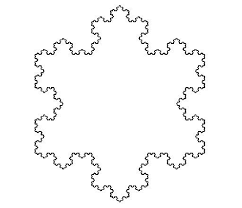
\includegraphics[width=0.5\linewidth]{geofr}}
\caption{Пример геометрического фрактала}
\label{ris:image}
\end{figure}

\item Алгебраические фракталы – самая обширная группа фракталов. Алгебраические фракталы получают с помощью нелинейных процессов в n-мерных пространствах. 

Пример алгебраического фрактала: множество Мандельброта.


\begin{figure}[H]
\center{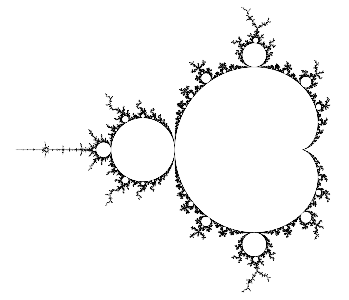
\includegraphics[width=0.5\linewidth]{anfr}}
\caption{Пример алгебраического фрактала}
\label{ris:image}
\end{figure}


\item Стохастические фракталы. Данные фракталы получаются, если в итерационном процессе менять хаотично некоторые параметры фрактала. Объекты, полученные таким образом, похожи на объекты реального мира – например, береговые линии.


\begin{figure}[H]
\center{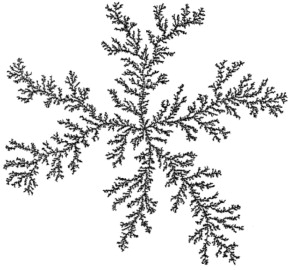
\includegraphics[width=0.5\linewidth]{stfr}}
\caption{Пример стохастического фрактала}
\label{ris:image}
\end{figure}

\end{enumerate}



По формальному признаку фракталы бывают: 
\\
\begin{enumerate}
\item связанные;


\begin{figure}[H]
\center{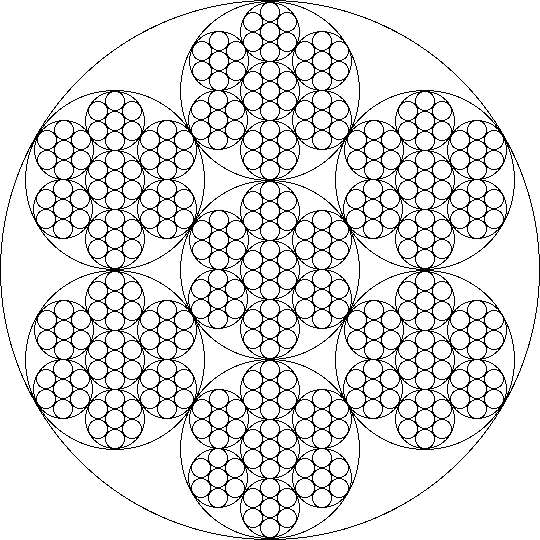
\includegraphics[width=0.5\linewidth]{ss}}
\caption{Пример связанного фрактала}
\label{ris:image}
\end{figure}

\item несвязанные.

\begin{figure}[H]
\center{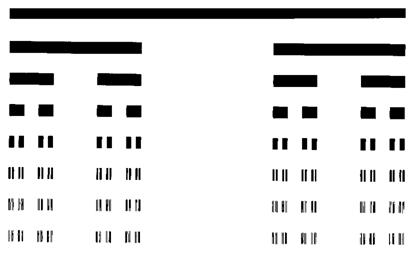
\includegraphics[width=0.5\linewidth]{nots}}
\caption{Пример несвязанного фрактала}
\label{ris:image}
\end{figure}

\end{enumerate}

По размерности фракталы бывают: 
\\
\begin{enumerate}
\item с целой размерностью;


\begin{figure}[H]
\center{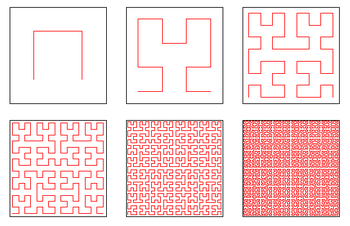
\includegraphics[width=0.5\linewidth]{crve}}
\caption{Кривая Пеано}
\label{ris:image}
\end{figure}

\item с дробной размерностью.


\begin{figure}[H]
\center{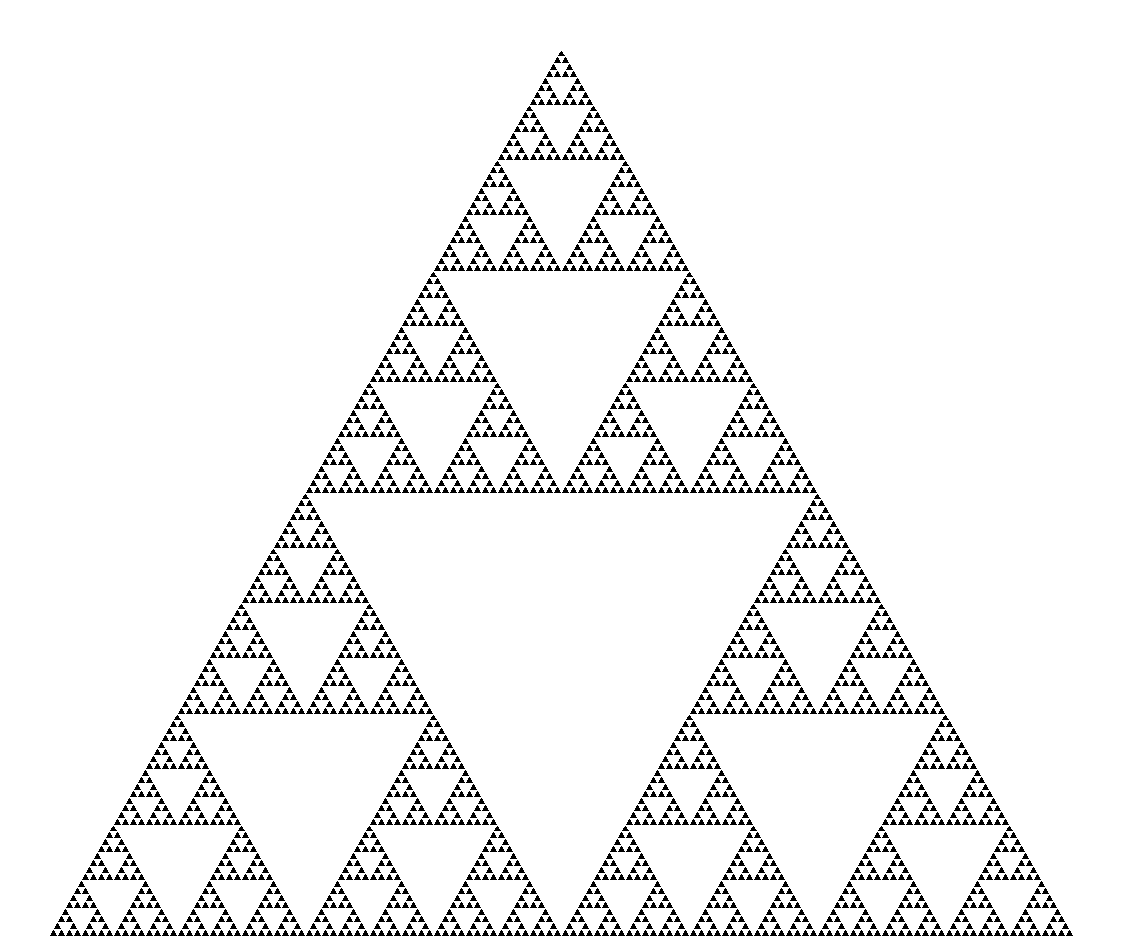
\includegraphics[width=0.5\linewidth]{s}}
\caption{Треугольник Серпинского}
\label{ris:image}
\end{figure}

\end{enumerate}

Помимо этого фракталы так же делятся на недетерминированные, к которым относятся геометрические и алгебраические фракталы, и на детерминированные (стохастические и алеаторные), линейные, строящиеся по линейному алгоритму, и нелинейные.
\\

В виду своей наглядности фракталы нашли свое применение в области компьютерной графики, но их так же можно применять и для баз данных. 
\\

Современные базы данных хранят огромное количество записей, описывающих те или иные объекты. Как правило, эти данные имеют некоторую структуру, которую мы можем использовать в своих целях.
\\
В базах данных в качестве самоподобной части фрактала выступают домены. 
\pagebreak
\subsection{Методы data mining}

Data mining – собирательное название совокупности методов обнаружения в сырых данных «скрытых» закономерностей и дальнейшей работы с ними.
\\

Основные задачи, решаемые с помощью data mining:
\begin{enumerate}
\item классификация – отнесение объекта к одному из непересекающихся множеств;

\begin{figure}[H]
\center{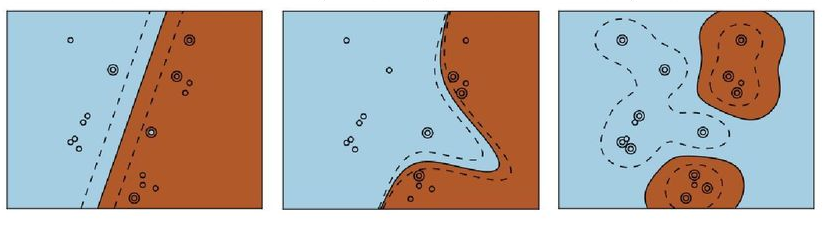
\includegraphics{class}}
\caption{Классификация}
\end{figure}

\item регрессия – установление зависимости непрерывных выходных данных от входных;

\begin{figure}[H]
\center{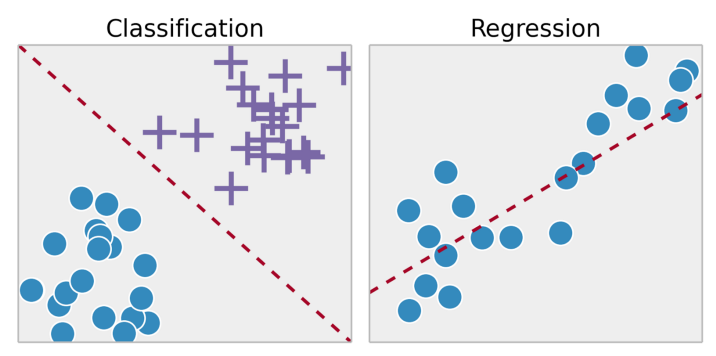
\includegraphics{reg}}
\caption{Регрессия}
\end{figure}


\item кластеризация – группировка объектов на основе их свойств;

\begin{figure}[H]
\center{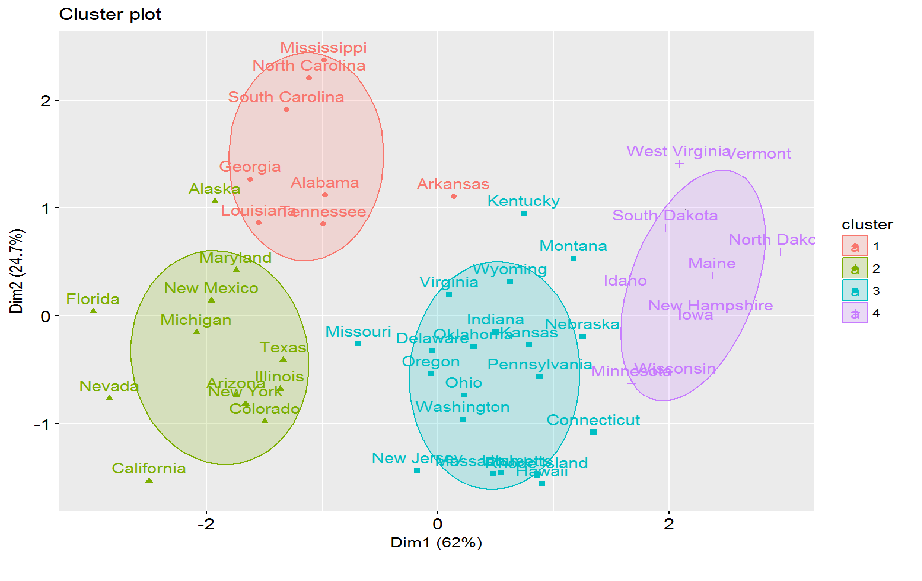
\includegraphics{clast}}
\caption{Кластеризация}
\end{figure}

\item ассоциация – выявление закономерностей между связанными событиями;

\item прогнозирование – оценка на основе уже имеющихся данных пропущенных или будущих значений;  

\item определение отклонений  – обнаружение данных, наиболее отличающихся от общего множества.
\end{enumerate}


\pagebreak
\subsection{Методы интеллектуального анализа данных}

Фракталы особенно показали свою эффективность в области data mining. Для обработки данных в работе использовались следующие фрактальные техники: кластеризация и понижение размерности.
\\

При кластеризации происходит разбиение элементов множества на группы в зависимости от их схожести. Самоподобие фракталов позволяет очень естественно определить кластеры, не ораничивая их какой-то конкретной формой.  При фрактальной кластеризации кластеры образуются, основываясь на фрактальной размерности: внутри кластера точки имеют большую степень самоподобия, чем вне его. При добавлении новых точек вычисляется новая фрактальная размерность и происходит перерасчет. Уже образованные кластеры могут разбиваться на новые или соединяться в один.
\\

При понижении размерности происходит исключение коррелирующих атрибутов отношения. Атрибуты, которые могут быть получены на основе других, исключаются из дальнейшей обработки. Для выявления повторяющихся данных используется свойство фрактальноц размерности, оценка степени свободы набора данных. 

\pagebreak

\subsection{Алгоритм фрактального поиска}

Для решения задачи фрактального поиска воспользуемся теорией реляционных баз данных. Ввёдем  основные термины.
\\

Домен – некоторое конечное множество данных, обозначается как $D_i$ , где i – номер домена. Отдельный элемент домена обознается как $d_i$,  где i – также номер домена.
\\

Полное декартово произведение множеств – набор всевозможных сочетаний из n элементов каждое, где каждый элемент берётся из своего домена. Описание:  $D_1 \times D_2 \times \dots \times D_n$.
\\

Отношение R – подмножество декартова произведения множеств  $D_1$,  $D_2$ \dots  $D_n$, необязательно различных. Описание: R $\subseteq$   $D_1 \times D_2 \times \dots \times D_n$. Число n называется степенью отношения.
\\

Атрибутом называют домен, входящий в отношение. Степень отношения определяет количество атрибутов в отношении. 
\\

Схемой отношения S называется перечень имён атрибутов данного отношения с указанием домена, к которому они относятся. Описание: $S_R$ = ($A_1, A_2, \dots A_n$.), $A_i$ $\subseteq$ $D_i$.
\\

Каждому имени атрибута $A_i$ ставится в соответствие множество $D_i$ — множество значений атрибута $A_i$, 1$\leq$i$\leq$n, D — объединение $D_i$, 1$\leq$i$\leq$n.  
\\

Отношение R со схемой S — это конечное множество отображений {$t_1$, $t_2$,…, $t_n$} из S в D; причем каждое отображение t должно удовлетворять следующему ограничению: t($A_i$) принадлежит $D_i$, 1$\leq$i$\leq$n. Эти отображения называются кортежами. 
\\

Из последнего определения видно, что отношение состоит из нескольких частей, кортежей. Именно кортеж несёт в себе информацию о структуре отношения.
\\

Алгоритм фрактального поиска рассматривает именно кортежи. Мы рассматриваем атрибуты кортежа как отдельные части, сохраняя при этом сведения о структуре в целом. 
\\

Так как каждый атрибут имеет конечное множество значений, множество значений набора атрибутов будет также иметь конечно. В этом случае можно предположить, что домены в отношении могут иметь идентичную структуру и одинаковые значения. 
\\

Принимая это предположение, возможно выделить домены в отношении, определить взаимосвязь атрибутов и фрактально сжать таблицу, сохранив при этом её структуру. Фрактальное сжатие поможет не только более компактно хранить имеющиеся данные, но и обнаружить в данных нетривиальные корреляции, полезные для дальнейшего анализа данных.
\\

Основная идея алгоритма фрактального поиска заключается в подборе такого множества доменов, которое не только полностью опишет структуру отношения, но и позволит представить данные в базе минимальным количеством записей. 
\\

\begin{figure}[H]
\center{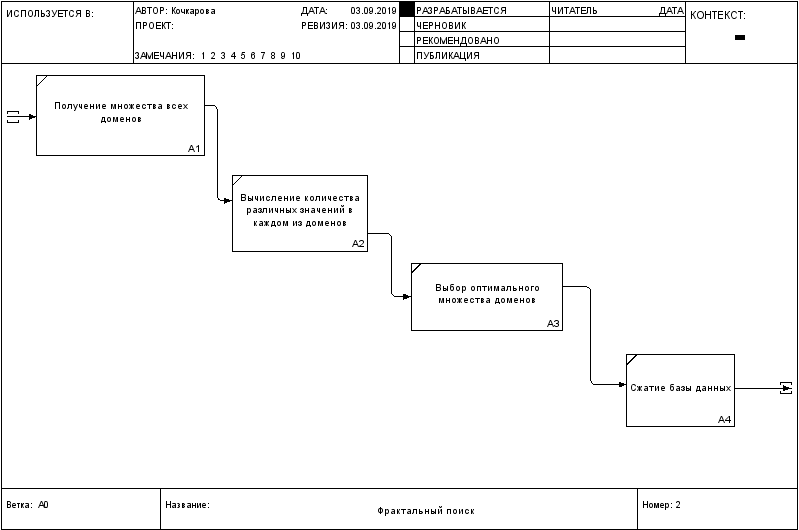
\includegraphics[width=1\linewidth]{02_A0}}
\caption{Диаграмма фрактального поиска}
\label{ris:image}
\end{figure}

\pagebreak

\subsection{Работа с доменами}

Пусть в нашей таблице имеется n атрибутов и в каждый домен входит k атрибутов, 1$\leq$k$\leq$n. 
\\

Количество различных доменов из k атрибутов: 
$C_n^k$ =  $(n!)\over (k!(n-k)!)$
\\

Количество всех возможных различных доменов: 
$\sum_{k=1}^n C_n^k$ =  $\sum_{k=1}^n$ $(n!)\over (k!(n-k)!)$

\begin{figure}[H]
\center{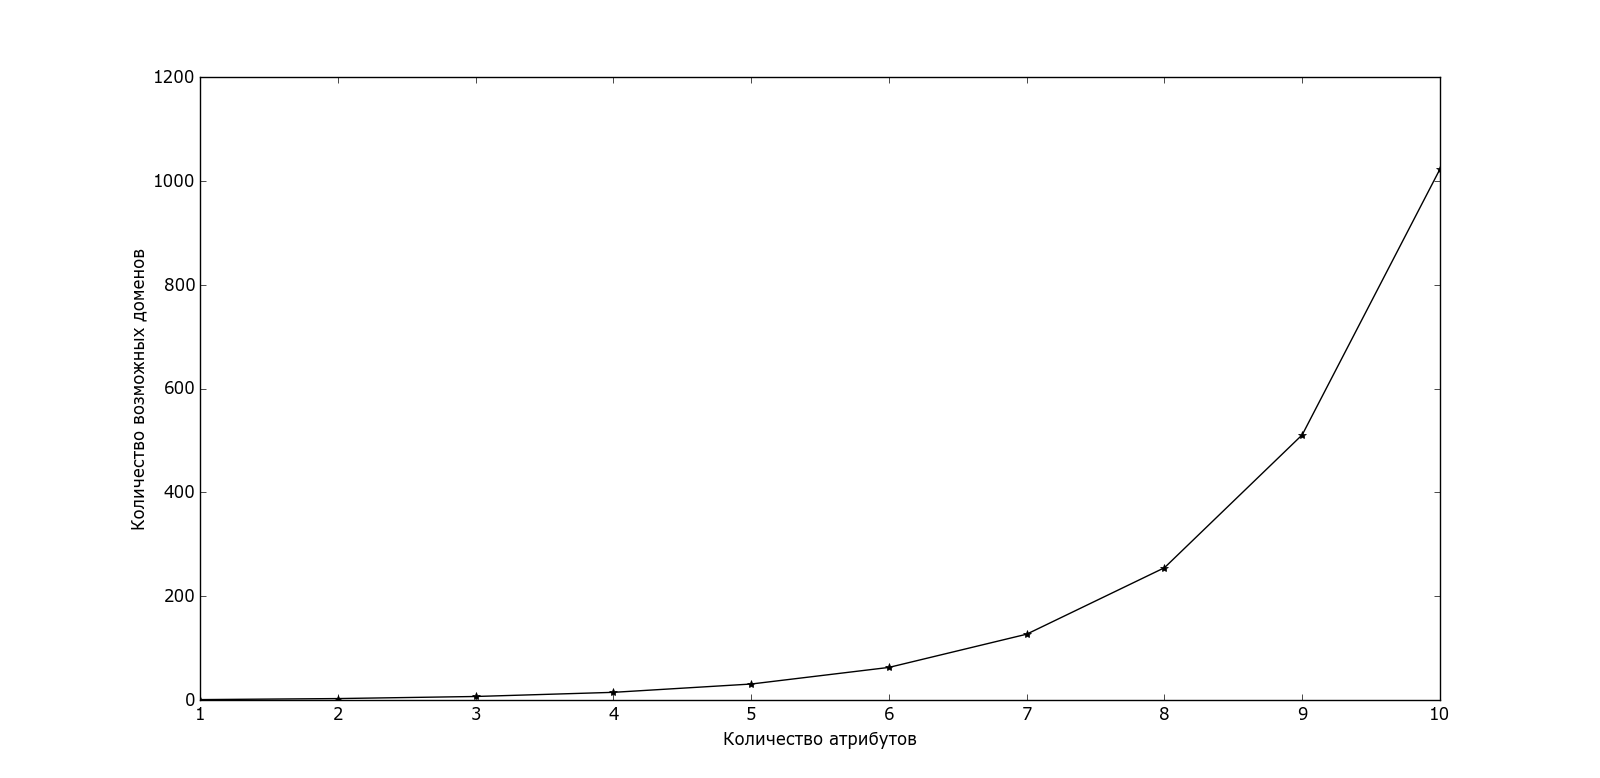
\includegraphics[width=1\linewidth]{size}}
\caption{Рост количества возможных доменов}
\end{figure}

Как видно из графика, с ростом количества атрибутов резко возрастает количество всех возможных доменов. Как правило, при формировании отношения число входящих в него атрибутов стараются ограничивать 15, что дает нам количество возможных структур не более 32767, однако при проектировании схемы базы данных могут и не придерживаться этого правила. Сложность во многом будет зависеть именно от количества атрибутов в таблице.
\\

Одной из важнейших характеристик домена является количество различных значений в нём. Чем меньше различных значений в домене, тем больше информации о структуре базы данных он отображает. Количество различных значений домена можно определить как произведение количества различных значений атрибутов, входяших в него, но на практике это число оказывается меньше. Поиск количества различных значений домена является самой затратной частью алгоритма фрактального поиска, поэтому имеет смысл ограничить размер доменов, чтобы сократить время выполнения данной части. 
\\

После того, как будет получено количество различных значений для каждего из множества доменов, необходимо получить оптимальное множество доменов. Оптимальное множество доменов полностью описывает таблицу и определяется как D = $D_1 + \dots + D_m$.

Оптимальное множество доменов должно удовлетворять следующим требованиям: 
\begin{enumerate}
\item все атрибуты должны быть в единственном экземпляре;
\item  сумма количества различных значений доменов должна быть минимальна.
\end{enumerate}

Алгоритм поиска оптимального множества является рекурсивной функцией: последовательно добавляются новые домены до тех пор, пока не будут просмотрены все атрибуты или пока количество различных значений доменов не превышает текущего минимума. При первом запуске минимум определяется как произведение количества атрибутов на количество строк, т.е. каждая ячейка считается уникальным значением. Если в базе данных существует несколько оптимальных множеств, данная реализация алгоритма выбирает первое из них.

\pagebreak
%главы конструкторской части
\section{Конструкторский раздел }

В данном разделе описаны основные объекты, используемые в системе.

\subsection{Основные структуры}

Для реализации программной системы был выбран язык программирования Python.  В качестве СУБД была использована MySQL. 

Используемые в системе классы: 
\begin{enumerate}
\itemатрибуты (Attribute);
\itemтаблица (Table);
\itemдомен (Domen);
\itemмножество всех доменов (DomenSearch);
\itemмножество оптимальных доменов (OptimalDomen).
\end{enumerate}

\begin{figure}[H]
\center{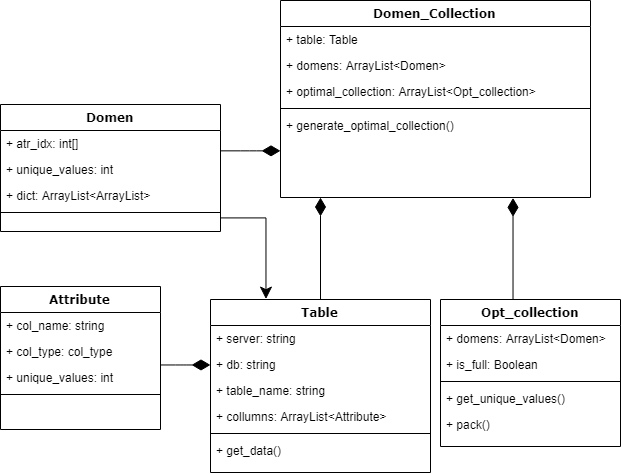
\includegraphics[width = 0.8\linewidth]{class_d}}
\caption{Диаграмма классов}
\end{figure}

Класс атрибута описывает столбец обрабатываемой таблицы. Класс содержит имя столбца, тип данных, который он содержит, а также количество уникальных значений. 
\\

\begin{figure}[H]
\lstinputlisting{attribute.py}
\caption{Класс атрибута}
\end{figure} 
 

Класс таблицы описывает обрабатываемую таблицу. Класс содержит имя столбца, её размер, а также лист атрибутов-столбцов. Помимо этого класс содержит методы получения данных.
\\

\begin{figure}[H]
\lstinputlisting{table.py}
\caption{Класс таблицы}
\end{figure} 

Класс домена описывает наименьший основной фрактальный объект, домен. Класс содержит лист индексов входящих в него атрибутов-столбцов, а также количество уникальных значений в данном домене. Класс включает в себя метод получения количества уникальных значений.
\\

\begin{figure}[H]
\lstinputlisting{domen.py}
\caption{Класс домена}
\end{figure} 
 
Класс множества всех доменов описывает алгоритмы работы с множеством доменов. Класс содержит лист индексов входящих в него атрибутов-столбцов, а также количество уникальных значений в данном домене. Класс включает в себя метод получения количества уникальных значений.

\begin{figure}[H]
\lstinputlisting{domen_collection.py}
\caption{Класс домена}
\end{figure} 
  

\pagebreak
%главы исследовательской части
\section{Технологический раздел }

В соответствии с поставленной задачей, проект должен быть доступен пользователю быстро и не требовать сложной установки.

В настоящее время все больше проектов используют браузер для отображения пользовательского интерфейса.

\subsection{Стек технологий}

Данное приложение разрабатывалось на основе Django, фреймворка для веб-приложений на языке Python. Фреймворк использует схему разделения данных MVC. Данный шаблон проектирования используется для разделения приложения, логики и пользовательского интерфейса, что позволяет модифицировать их отдельно друг от друга.
\\

MVС состоит из трех компонентов: модели (Model), представления (View) и контроллера (Controller).  

\begin{figure}[H]
\center{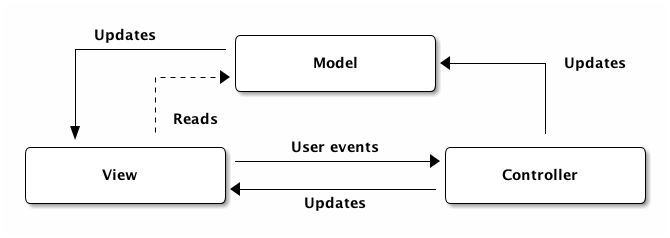
\includegraphics[width = 1\linewidth]{mvc}}
\caption{Паттерн MVC}
\end{figure}

Модель описывает используемые в приложении данные и реагирует на команды контроллера. Представление отвечает за отображение данных модели пользователю, реагируя на изменения модели. Контроллер обрабатывает действия пользователя и взаимодействует с моделью.
\pagebreak

\subsection{Взаимодействие с ПО}



\pagebreak

%вывод и библиография
\section{Заключение}

В данном курсовом проекте были успешно реализованы все поставленные задачи. Для алгоритма было разработано веб-приложение с простым интерфейсом.
Разработанный алгоритм может быть использован в качестве инструмента для интеллектуального анализа баз данных.
\\

Данный алоритм имеет несколько перспективных направлений развития:
\begin{enumerate}
\item модификация алоритма, связанная с предварительным понижением фрактальной размерности баз данных
\item разработка полностью параллельного алгоритма фрактального поиска
\end{enumerate}

\section*{Список использованных источников}
\addcontentsline{toc}{section}{Список использованных источников}

\begin{thebibliography}{3}
\bibitem{0} Т.Ю. Лымарь, Т.С. Мантрова, Н.Ю. Староверова "АЛГОРИТМ ФРАКТАЛЬНОГО ПОИСКА  В РЕЛЯЦИОННЫХ БАЗАХ ДАННЫХ"
\end{thebibliography}

\end{document}